\chapter{Project Management}
\label{Chapter:ProjectManagement}
Due to the extensive length and size of this project, consideration into how the project can be effectively
managed was very important to project success. The following sections will discuss the chosen design and development methodologies, providing justification for each choice and will also look at the risks affecting project progress and success.

\section{Design Approach}
The design approach adopted for system UI was component-driven design. Component-driven design allowed more focus and thought to be given for each component. Going with this approach was greatly beneficial to the project as it meant components were designed independently of each other. Another advantage of using this methodology is that it provides the opportunity to re-use designed components across multiple applications. 

For algorithm design, an Agile approach was used. Agile methodologies provided flexibility when researching and designing chosen algorithms. Over the course of the project, numerous algorithms were considered and with the flexibility provided by this approach meant any required changes to algorithm design were prompt.

\section{Software Development Methodology}
Agile methodologies were employed for project development. This, coupled with component-driven design meant enabled components to be designed, built and tested seamlessly. Agile techniques were used due to their flexibility in handling evolving requirements. Due to the project length, it was important to adopt an adaptive development methodology. Building the system using Agile techniques eases the integration of new system components, and increases the efficacy of unit testing. Another reason that an agile approach was chosen was that as development progresses, issues will arise which may not have been accounted for previously. Adapting to these issues, and evolving requirements would not be possible with a plan-driven approach such as Waterfall. Given their linear nature, requirements refinement is much more difficult hence an agile approach provides a way of handling changing requirements. 

One fact that must be brought to light is that agile methodologies do not focus on documentation as much as a plan-driven approaches. As documentation is a key part of the non-functional requirements of this project, a modified version of the agile approach, one where documentation is important, was used. In addition to this, rapid prototype development was also employed to cope with the overlapping of development and testing, allowing for quick component prototypes to be created and tested. To counteract the effects of reduced documentation, regular meetings were held with with project supervisor to ensure that project goals remained on track. Similarly, within the project group itself weekly meetings were held. Much like daily scrums, these meetings again reinforced project goals and provided a platform where next steps and progress blockers could be discussed.

\section{Project Timeline}
The proposed project timeline, composed during the project specification and visible in Figure \ref{fig:timeline} has remained largely unchanged. Given how the timeline was designed, providing generous float time to each activity, few minor changes were made to the original plan. To accommodate for the increased workload faced by team members in Term 2, work on the final report was delayed until March. Although this at first seems like a major delay, the 14 week period initially assigned for writing this report was purposefully made longer than required to accommodate for unforeseen circumstances that would affect the task. Subsequently, draft completion dates and feedback cycles were also pushed back. The implementation for each algorithm ran longer than originally planned. This again did not affect the overall plan as these tasks were already overlapping and as each algorithm was implemented by a different team member, full task parallelisation was possible, meaning the completion date for the final algorithm was successfully met.

\begin{figure}[H]
  \centering
  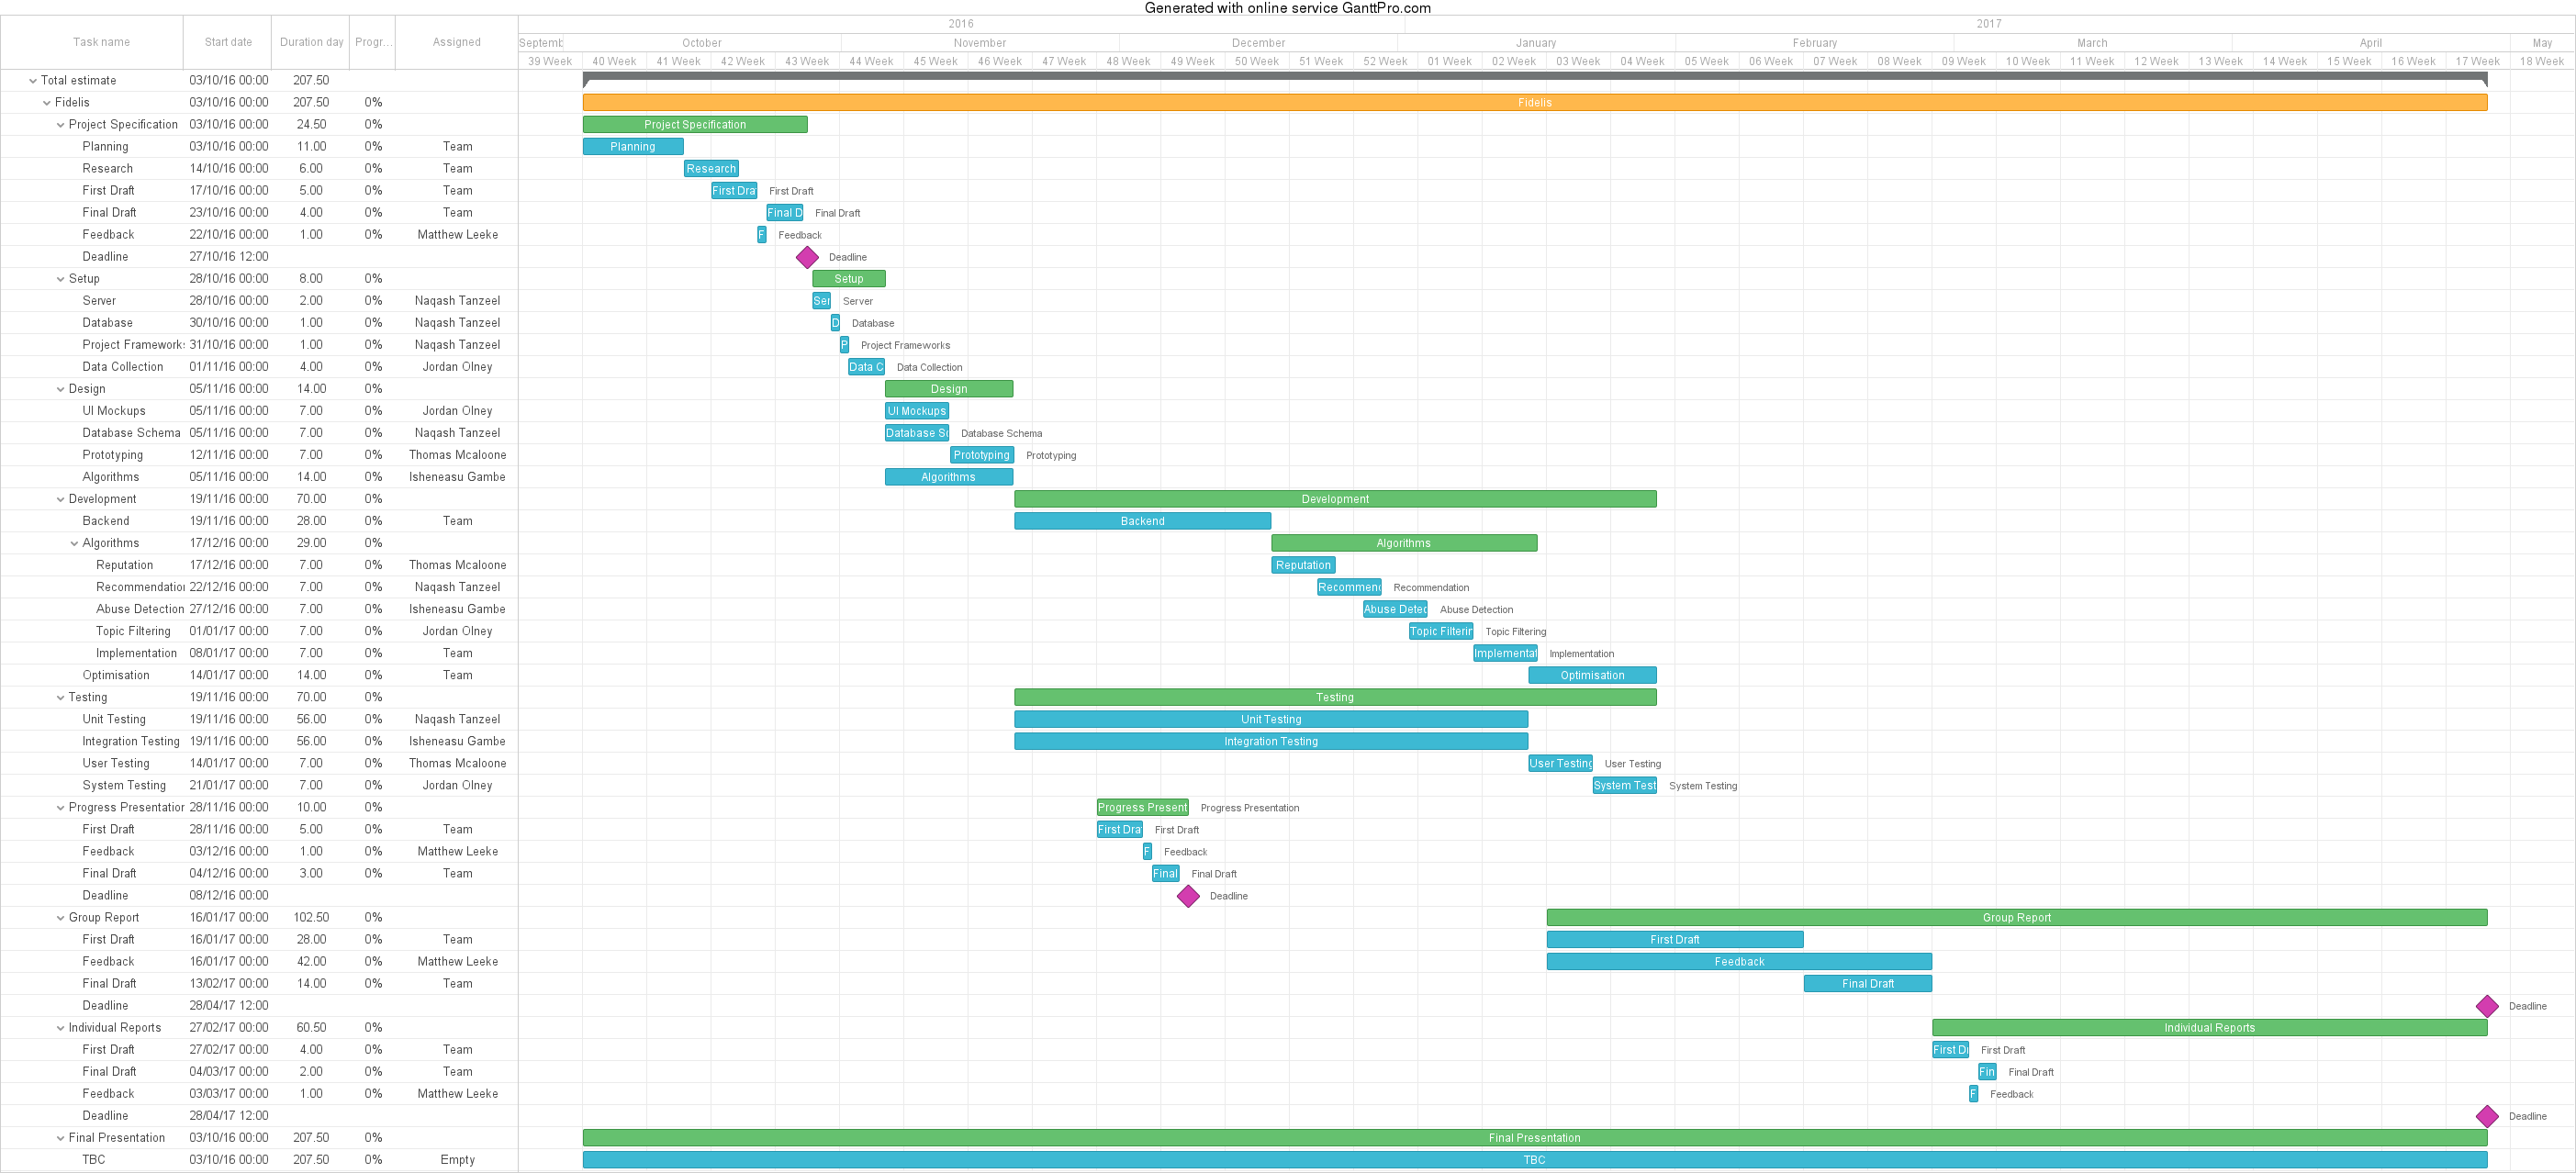
\includegraphics[width=1.0\textwidth]{Images/ProjectManagement/timeline}
  \caption{Project timeline} 
  \label{fig:timeline} 
\end{figure}

\section{Tools and Techniques}
A range of third-party tools and technologies were employed to successfully manage and develop the project. These tools have an immense amount of support and resources available online. As a result less time is spent `firefighting', solving issues, and `reinventing the wheel', hence allowing more time to be spent on developing the unique aspects of the projects. Using existing frameworks and tools also provides the added benefit that fundamental features and functionality is implemented by the third-party provider but can be taken advantage of by the developer. The tools employed were used for different tasks, either for developing the project or managing it to ensure a smooth operation, each of which are discussed in further detail below.

\subsection{Development}
\begin{figure}[H]
	\centering
	\begin{subfigure}[t]{0.2\linewidth}
		\centering
		
\includegraphics[width=\linewidth]{Images/Generic/Icons/Laravel}
		\caption{Laravel 5}\label{fig:Laravel}		
	\end{subfigure}
	\quad
	\begin{subfigure}[t]{0.2\linewidth}
		\centering
		
\includegraphics[width=\linewidth]{Images/Generic/Icons/HTML_5}
		\caption{HTML 5}\label{fig:HTML_5}
	\end{subfigure}
    \quad
	\begin{subfigure}[t]{0.2\linewidth}
		\centering
		
\includegraphics[width=\linewidth]{Images/Generic/Icons/CSS_3}
		\caption{CSS 3}\label{fig:CSS_3}
	\end{subfigure}
    \quad
	\begin{subfigure}[t]{0.2\linewidth}
		\centering
		
\includegraphics[width=\linewidth]{Images/Generic/Icons/JavaScript}
		\caption{JavaScript}\label{fig:JavaScript}
	\end{subfigure}
    \quad
	\begin{subfigure}[t]{0.2\linewidth}
		\centering
		
\includegraphics[width=\linewidth]{Images/Generic/Icons/PHP_7}
		\caption{PHP 7}\label{fig:PHP_7}
	\end{subfigure}
	\quad
	\begin{subfigure}[t]{0.2\linewidth}
		\centering
		
\includegraphics[width=\linewidth]{Images/Generic/Icons/MySQL}
		\caption{MySQL}\label{fig:MySQL}		
	\end{subfigure}
	\quad
	\begin{subfigure}[t]{0.2\linewidth}
		\centering
		
\includegraphics[width=\linewidth]{Images/Generic/Icons/jQuery}
		\caption{jQuery}\label{fig:jQuery}
	\end{subfigure}
    \quad
	\begin{subfigure}[t]{0.2\linewidth}
		\centering
		
\includegraphics[width=\linewidth]{Images/Generic/Icons/Apache}
		\caption{Apache}\label{fig:Apache}
	\end{subfigure}
	\caption{Development Tools Employed}\label{fig:DevelopmentTools}
\end{figure}

A wide range of technologies were used for the development of the project, some of which are shown in figure \ref{fig:DevelopmentTools}. Research into each of these technologies along with their advantages and disadvantages is provided in section \ref{Section:Technologies}. Section \ref{Chapter:Implementation} further discusses some of the core technologies such as Laravel, PHP, MySQL, jQuery and provides reasons for their use \cite{Laravel:Home, PHP:Home, MySQL:Home, jQuery:Home}. In addition to these core technologies, several smaller tools and technologies were also used. The majority of the user interface was developed using HTHML 5, although some of this was generated using the Laravel Blade engine, and styled using Bootstrap or custom Cascading Style Sheets \cite{W3:HTML5, Bootstrap:Home, W3:CSS}. Majority of the backend development was carried out using the popular scripting language PHP but some of this was also automatically generated using syntax provided by the Laravel Blade engine \cite{PHP:Home, Laravel:Blade}. 

\subsection{Management}
\begin{figure}[H]
	\centering
	\begin{subfigure}[t]{0.15\linewidth}
		\centering
		\includegraphics[width=\linewidth]{Images/Generic/Icons/PHPStorm}
		\caption{PhpStorm}\label{fig:PHPStorm}		
	\end{subfigure}
	\quad
	\begin{subfigure}[t]{0.15\linewidth}
		\centering
		
\includegraphics[width=\linewidth]{Images/Generic/Icons/Github}
		\caption{Github}\label{fig:Github}
	\end{subfigure}
    \quad
	\begin{subfigure}[t]{0.15\linewidth}
		\centering
		
\includegraphics[width=\linewidth]{Images/Generic/Icons/DigitalOcean}
		\caption{DigitalOcean}\label{fig:DigitalOcean}
	\end{subfigure}
    \quad
	\begin{subfigure}[t]{0.15\linewidth}
		\centering
		
\includegraphics[width=\linewidth]{Images/Generic/Icons/Wunderlist}
		\caption{Wunderlist}\label{fig:Wunderlist}
	\end{subfigure}
    \quad
	\begin{subfigure}[t]{0.15\linewidth}
		\centering
		
\includegraphics[width=\linewidth]{Images/Generic/Icons/Trello}
		\caption{Trello}\label{fig:Trello}
	\end{subfigure}
	\caption{Management Tools Employed}\label{fig:ManagementTools}
\end{figure}

All the code written throughout the development process was done using an IDE provided by JetBrains called PhpStorm \cite{JetBrains:PHPStorm}. PhpStorm provides syntax highlighting, code completion, and numerous other features for all major web development technologies. Optional plugins can be installed which provide support for even more technologies, as done for Laravel \cite{JetBrains:PHPStorm}. PhpStorm also provides integrated support for Git which was used to provide version control for all the code written. This allowed files to be added to Git as soon as they were created so they would not be omitted from commits, causing inconsistencies \cite{JetBrains:PHPStorm}. The use of Github allowed code to be backed up online, in case of a hardware failure, so it could be replicated onto another machine easily \cite{Github:Home}. This was particularly useful when deploying the code from the development server to the production server hosted by DigitalOcean\cite{DigitalOcean:Home}. As soon as a feature was fully implemented, it could be pushed up to the Github servers allowing for the changes to be fetched by the production server just by issuing a single command. 

\begin{figure}[H]
	\centering
	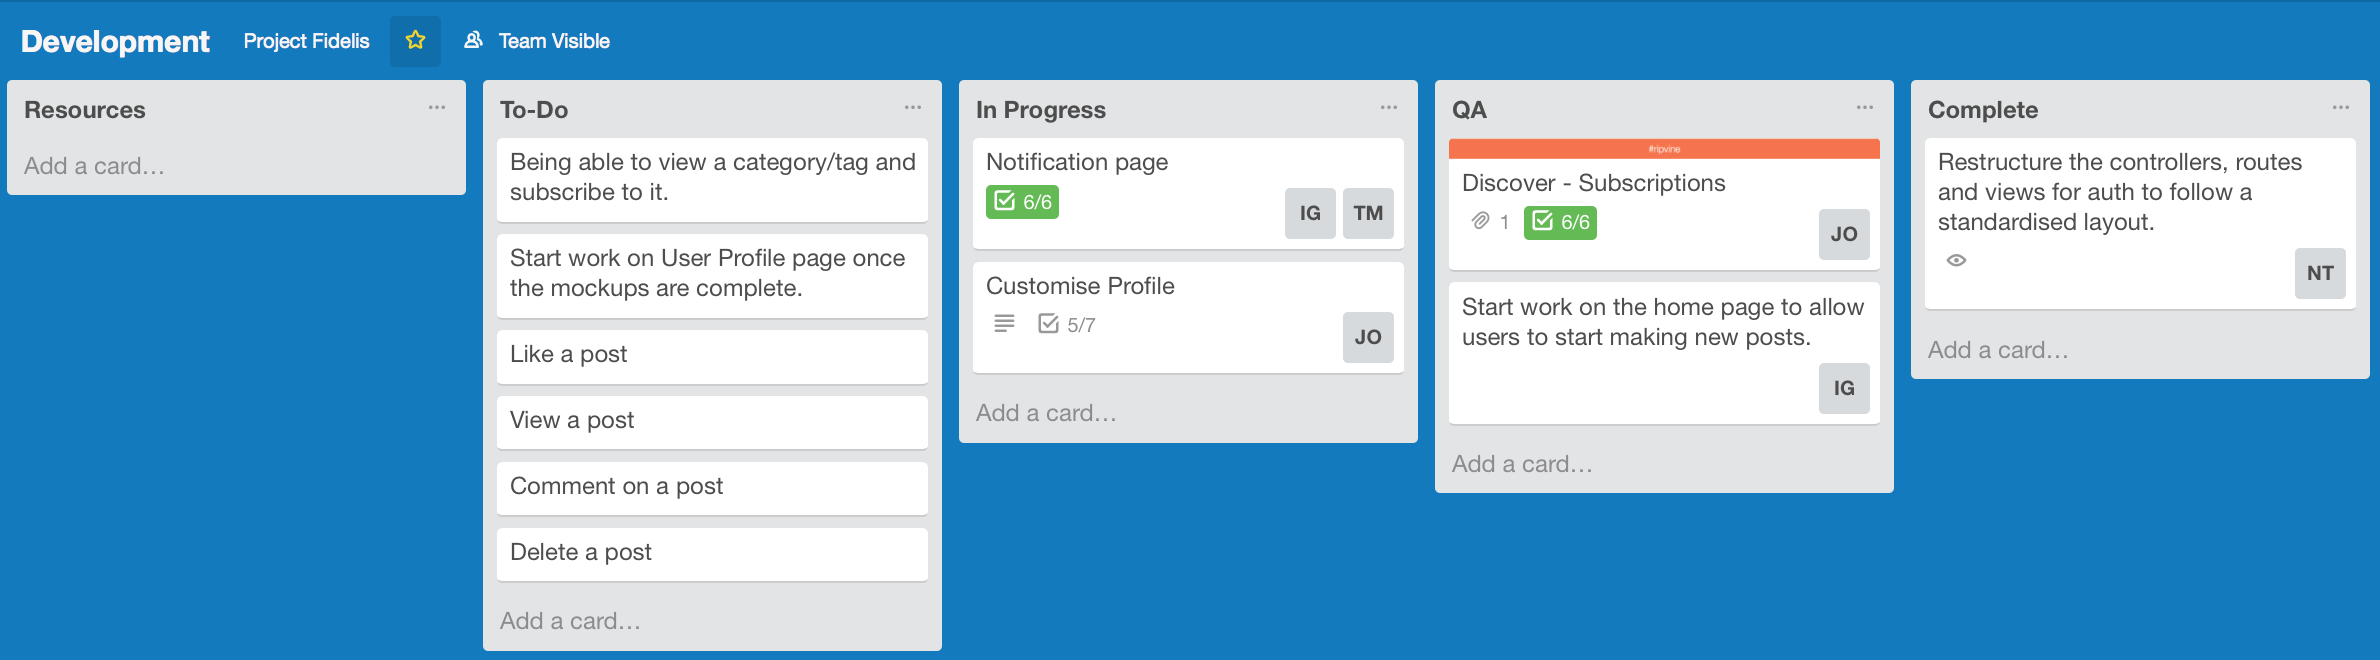
\includegraphics[width=1.0\textwidth]{Images/ProjectManagement/Trello}
	\caption{Trello: Project Work Breakdown Structure} \label{fig:Trello_WBS}
\end{figure}

A number of desktop and web applications were used to keep track of the daily development progress and any remaining work that needed to be completed. Wunderlist was used to keep track of daily tasks that needed to be completed whereas Trello, was used to keep an overall development log of all the features that were to be implemented \cite{Wunderlist:Home, Trello:Home}. Figure \ref{fig:Trello_WBS} shows just one of the boards, namely development tasks, used to keep track of progress. These were strictly for the developer and hence to communicate this progress, emails and face to face meetings were used to update the project supervisor and stakeholders. All the tools discussed are illustrated in figure \ref{fig:ManagementTools}.

\section{Risk Management}
Undertaking a project of this length, with the given time-scale and the nature of any software development project it was imperative that proper risk management be conducted to minimise major risks affecting project completion. Risks affecting developers, software, hardware, data and third party services were considered and mitigated against.

\subsection{Developer}
Project developers are crucial to project success. As with any software development project, the importance in understanding and managing risks that may affect developers cannot be undervalued. One of the main risks affecting any developer is their ability to perform the tasks they are assigned to. Illness, commitments to other work assignments or an inability to complete a given task can severely hinder project progress. To prevent any such occurrence, all developers were paired so that in the event that developer $A$ was unable to complete a task, developer $B$ would be able to understand and complete this task. Going beyond this, it was highly encouraged amongst the team to be aware of what other members were working on. This essentially meant that any developer was able to pick up tasks being handled by another developer. Additionally to this, effective communication channels were established within the team. This supported the idea of paired development as it made it easy for developers to work together, and also meant that potential issues were swiftly identified and dealt with.

\subsection{Hardware}
All development has been done using personal computers, so the only hardware relied upon during the project were these devices. Along with other work and personal use, each device was used heavily, and was therefore prone to failure. To mitigate against this, version control software was used to maintain functioning back-ups of all development work. Namely, Github was used for this purpose. Github allows ``snapshots'' of the functioning system to be taken, making data retrieval in the event of hardware failure very convenient and easily. In addition to this, each developer kept a copy of their work on the Computer Science Department lab machines. These two approaches covered the occurrence of single and multiple device failure.

\subsection{Data}
Data security is important to any project where user data is collected. Exposing user data could leave the system and developers liable to penalties or criminal charges from relevant regulatory bodies. For this reason, it is important to ensure that in the case that user data is exposed, safeguards are in place to protect both the users and developers. To avoid storing plain-text user credentials, user passwords are hashed before being stored in the database, making it almost impossible for anyone to decrypt the data within a reasonable period of time. During the registration process, minimal information is requested from the user. When registering, the only information requested from the user is their name and email address. This minimal approach on user information lessens the amount of sensitive data held on users. Password-protecting the database added an extra layer of database security, minimising the chances of unauthorised access to any of the data.

Another piece of data that needs to be protected is any content that is uploaded by the user. Public user profiles are accessible to anyone on Fidelis, even to unregistered users. To provide users with the option of increased privacy, the user has the option to make their account private. This makes their content accessible only to their followers.

\subsection{Third Party Services}
The Twitter API is used to collect data for training a model for automatic post categorisation. This falls under content filtering, one of the core Fidelis functionalities. Were this service to fail, it would make the process of collecting training data very difficult and cumbersome. In the event that such a failure would occur, alternative datasets were collected. A number of public datasets for natural language processing are available online. The Blog Authorship Corpus is a public dataset containing 681288 blog posts from 2004 \cite{dataset:blogs}. This, along with several other datasets \cite{dataset:all} were available as fall-back training datasets.

The API has a rate limit on the number of tweets that can be fetched, permitting 180 tweets per 15 minute window \cite{twitter-api:rates}. This rate puts a restriction on how many tweets can be collected daily, and inefficient tweet collection can therefore lead to not enough data being collected. This would in turn hamper the training of the model. To maximise the number of tweets collected, data collection began early on in the project and a DigitalOcean droplet was setup, allowing automated data collection on the server.
